\subsection*{d. Toda la información de los clientes del segmento Consumer que realizaron una orden con modo de envío Second Class y que no viven en Nevada.}

Primero seleccionamos de \textit{customer} a los clientes del segmento \textit{Consumer} que no viven en \textit{Nevada}. Después seleccionamos de la tabla \textit{orders} las órdenes con modo de envío \textit{Second Class} y proyectamos solamente el id de los clientes que las realizaron. Finalmente, realizamos un join natural entre ambos resultados, para que solamente nos queden los clientes que cumplen todas las condiciones, junto con si información completa.

Expresión:
\begin{equation}
\sigma_{segment = \text{'Consumer'} \, \wedge \, state \neq \text{'Nevada'}}(customer) \bowtie \pi_{customerid}\left(\sigma_{shipmode = \text{'Second Class'}}(orders)\right)
\end{equation}

Resultados obtenidos:

\begin{figure}[h!]
\centering
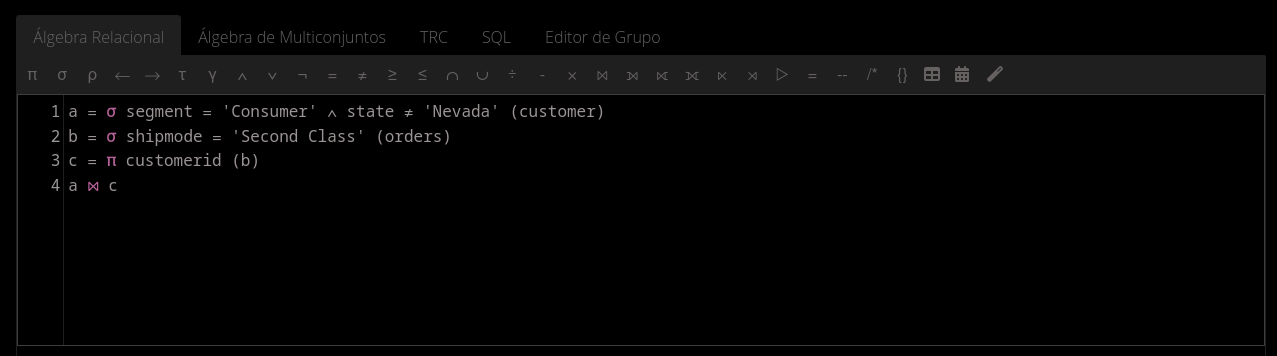
\includegraphics[width=0.8\textwidth]{imagenes/2d(1).png}
\caption{Consulta}
\end{figure}

\begin{figure}[h!]
\centering
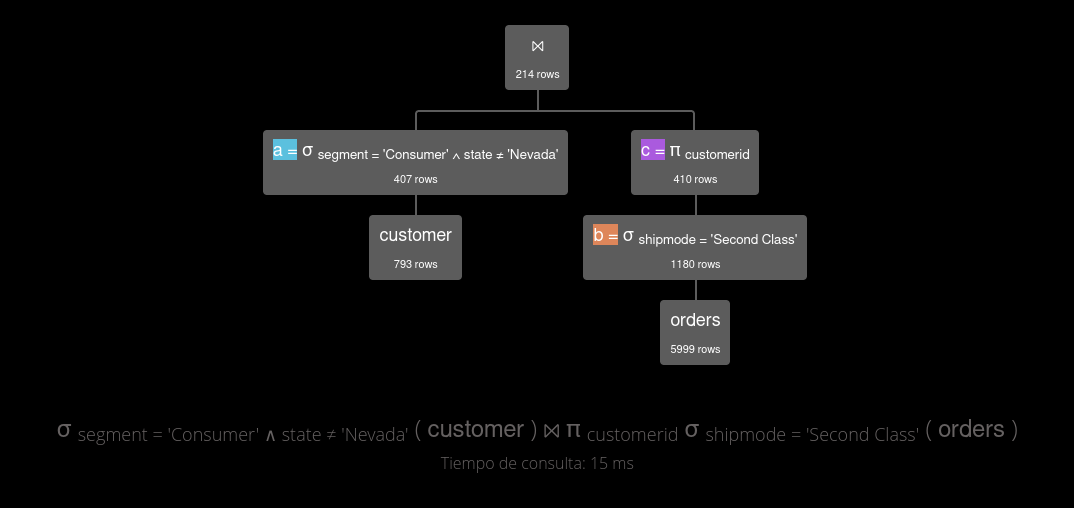
\includegraphics[width=0.8\textwidth]{imagenes/2d(2).png}
\caption{Árbol de consulta.}
\end{figure}

\begin{figure}[h!]
\centering
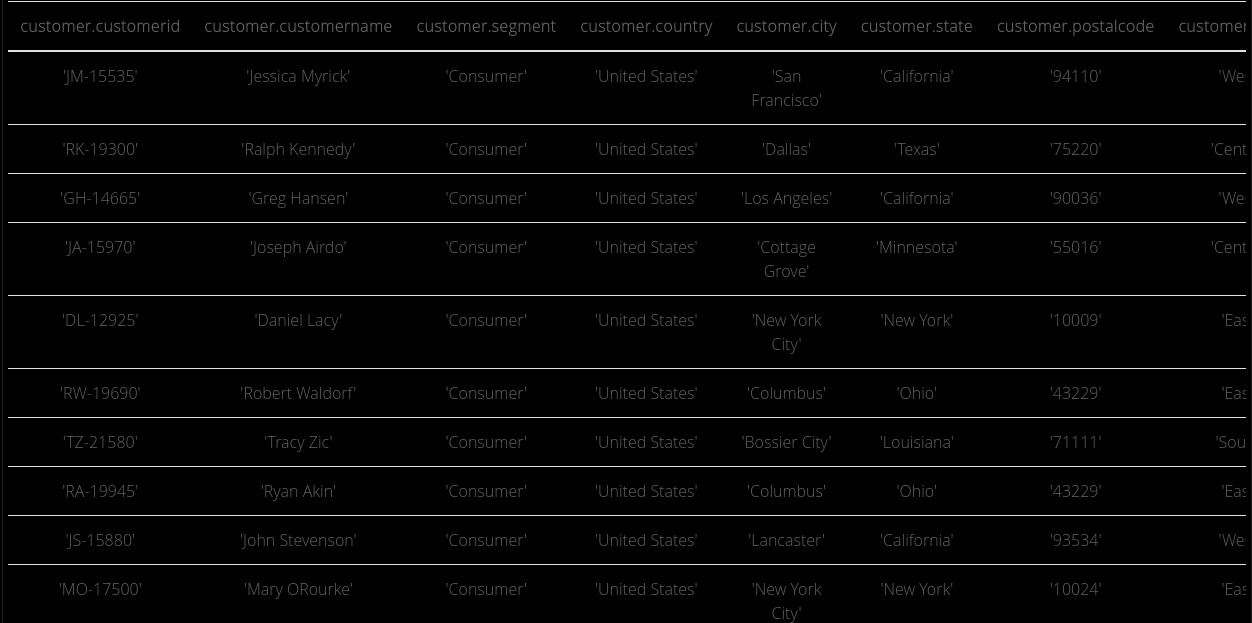
\includegraphics[width=0.8\textwidth]{imagenes/2d(3).png}
\caption{Resultado de consulta.}
\end{figure}